% arara: pdflatex: {files: [MathSACpr2014]}
% !arara: indent: {overwrite: yes}
\chapter{Facilities and Support}
\begin{flushright}
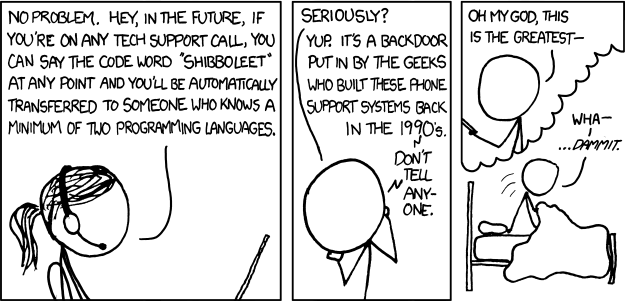
\includegraphics[width=8cm]{xkcd-806-tech_support-punchline}\\
\url{http://xkcd.com}
\end{flushright}
\section{Describe how classroom space, classroom technology, laboratory space
and equipment impact student success.}

Over the past few years, efforts by the college to create classrooms containing
the same basic equipment has helped tremendously with consistency issues.  The
nearly universal presence of classroom podiums with attendant Audio Visual (AV) devices is
considerably useful.  For example, many instructors use computer-based
calculator emulators when instructing their students on calculator use---this
allows explicit keystroking examples to be demonstrated that were not possible
before the podiums appeared; the document cameras found in most classrooms are
also used by most mathematics instructors.     Having an instructor computer with
internet access has been a great help as instructors have access to a wide
variety of tools to engage students, as well as a source for quick answers when
unusual questions arise.  

Several classrooms on the Sylvania campus have Starboards  or Smart Boards
integrated with their AV systems.  Many mathematics instructors use these tools
as their primary presentation vehicles;  documents can be preloaded into the
software and the screens allow instructors to write their work directly onto
the document.  Among other things, this makes it easy to save the work into pdf
files that can be accessed by students outside of class.  This equipment is not
used as much on the other campuses, but there are instructors on other campuses
that say they would use them if they were widely available on their campus.

A few instructors have begun creating lessons with LiveScribe technology.  The
technology allows the instructor to make an audio/visual record of their
lecture without a computer or third person recording device; instructors can 
post a `live copy' of their actual class lecture online.  The students  do not 
simply see a static copy of the
notes that were written;  the students see the notes emerge as they were being
written and they hear the words that were spoken while they were written.  The
use of LiveScribe technology is strongly supported by Disability Services, and
for that reason alone continued experimentation with its use is strongly
encouraged.

Despite all of the improvements that have been made in classrooms over the past
few years, there still are some serious issues.

Rooms are assigned randomly, which often leads to mathematics classes being
scheduled in rooms that are not appropriate for a math class. For example,
scheduling a math class in a room with individual student desks creates a lot
of problems; many instructors have students take notes, refer to their text,
and use their calculator all at the same time and there simply is not enough
room on the individual desktops to keep all of that material in place.  More
significantly,  this furniture is especially ill-suited for group work.  Not
only does the movement of desks and sharing of work exacerbate the materials
issue (materials frequently falling off the desks), students simply cannot
share their work in the efficient way that work can be shared when they are
gathered about tables.  It would be helpful if all non-computer-based math
classes could be scheduled in rooms with tables.

Another problem relates to an inadequate number of computerized classrooms and
insufficient space in many of the existing computerized classroom;  both of
these shortages have greatly increased due to Bond-related construction.
Several sections of MTH 243 and MTH 244 (statistics courses), which are
normally taught in computerized classrooms, \emph{have} been scheduled in regular
classrooms.  Many of the statistics courses that were scheduled in
computerized classrooms have been scheduled in rooms that seat only 28, 24, or
even 20 students.  When possible, we generally limit our class capacities at 34
or 35.  Needless to say, running multiple sections of classes in rooms well
below those capacities creates many problems.  This is especially  problematic
for student success, as it hinders students'  ability to register due to
undersized classrooms.

Finally, the computerized classrooms could be configured in such a way that
maximizes potential for meaningful student engagement and minimizes potential
for students to get off course due to internet access.  We believe that all
computerized classrooms need to come equipped with software that allows the
instructor control of the student computers such as LanSchool Classroom
Management Software.   The need for this technology is dire; it will reduce or
eliminate students being off task when using computers, and it will allow
another avenue to facilitate instruction as the instructor will be able to
`see' any student computer and `interact' with any student computer.  It can
also be used to solicit student feedback in an anonymous manner.  The gathering
of anonymous feedback can frequently provide a better gauge of the general
level of understanding than activities such as the traditional showing of
hands.

\subsection{Recommendations}
\recommendation{All mathematics classes should be scheduled in rooms that are either
computerized (upon request) or have multi-person tables (as opposed to
individual desks).}

\recommendation{All computerized classrooms should have at least 30, if not 34, individual work
stations.}

\recommendation{An adequate number of classrooms on all campuses should be equipped with
Smartboards so that all instructors who want access to the technology can teach
every one of their classes in rooms equipped with the technology.}

\recommendation{The computer image for all computerized classrooms should include software that
allows the instructor computer complete and direct access to each student
computer. }

\fixthis{ add one about LiveScribe?}

\section{Describe how students are using the library or other
outside-the-classroom information resources.  }
We researched this topic by conducting a stratified sampling method
survey of 976 on-campus students and 291 online students; the participants were
chosen in a random manner.  We gave scantron surveys to the on-campus students
and used SurveyMonkey for the online students. We found that students are
generally knowledgeable about library resources and other outside-the-classroom
resources.  The complete survey, together with its results, is given in
\vref{app:sec:resourcesurvey}; we have summarized our comments to some of the 
more interesting questions below.

\begin{enumerate}[label=Q\arabic*.,font=\bf]
  \item Not surprisingly, library resources and other campus-based resources
    are used more frequently by our on-campus students than by our online
    students. This could be due to less frequent visits to campus for online
    students and/or online students already having similar resources available
    to them via the internet. 
  \item We found that nearly 70\% of instructors include resource information
    in their syllabi.  This figure was consistent regardless of the level of
    the class (DE/transfer level) or the employment status of the instructor
    (full/part-time).

    We found that a majority of our instructors are using online resources to
    connect with students. Online communication between students and
    instructors is conducted across many platforms such as instructor websites,
    Desire2Learn, MyPCC, online graphing applications, and online homework
    platforms.  

    We found that students are using external educational websites such as \href{https://www.khanacademy.org/}{Khan Academy}, 
    \href{http://patrickjmt.com/}{PatrickJMT}, \href{http://www.purplemath.com/}{PurpleMath}, and \href{http://www.youtube.com/}{YouTube}.  The data suggest online
    students use these services more than on-campus students.
  \item The use of online homework (such as WeBWorK,  MyMathLab, MyStatLab, and
    ALEKS) has grown significantly over the past few years. However, the data
    suggests that significantly more full-time instructors than part-time
    instructors are directing their students towards these tools (as either a
    required or optional component of the course).  Additionally, there is a
    general trend that online homework programs are being used more frequently
    in online classes than in on-campus classes.  Both of these discrepancies
    may reflect the need to distribute more information to faculty about these
    software resources.
  \item The math SAC needs to address whether or not we should be requiring
    students to use online resources that impose additional costs upon the
    students and, if so, what would constitute a reasonable cost to the
    student.  To that end, our survey asked if students would be willing to pay
    up to \$35 to access online homework and other resources.   We found that
    online students were more willing to pay an extra fee than those enrolled
    in on-campus classes. 
\setcounter{enumi}{6}
  \item The PCC mathematics website offers a wealth of materials that are
    frequently accessed by students. These include course-specific supplements,
    calculator manuals, and the required Calculus I lab manual; all of these
    materials were written by PCC mathematics faculty.  Students may print
    these materials for free from any PCC computer lab. The website also links
    to PCC-specific information relevant to mathematics students (such as
    tutoring resources) as well as outside resources (such as the Texas
    Instruments website).  
    \setcounter{enumi}{8}
  \item In addition to the previously mentioned resources we also encourage
    students to use resources offered at PCC such as on-campus Student Learning
    Centers, online tutoring, Collaborate, and/or Elluminate. A significant
    number of students registered in on-campus sections are using these
    resources whereas students enrolled in online sections generally are not.
    This is not especially surprising since on-campus students are, well, on
    campus whereas many online students rarely visit a campus . 
    \fixthis{comment below}
    % Three out of four of the resources listed are on line, but you're telling
    % me the on-campus students use them more.  I think I'm missing something
    % here.
\end{enumerate}
\subsection{Recommendations}
\recommendation{The majority of our data suggests that students are using a variety of
resources to further their knowledge. We recommend that instructors continue to
educate students about both PCC resources and non-PCC resources. We need to
uniformly encourage students to use resources such as online tutoring, student
learning centers, Collaborate, and/or Elluminate; this includes resource
citations in each and every course syllabus.}

\recommendation{A broader education campaign should be engaged to distribute information to
part-time faculty regarding online homework such as WeBWorK, MyMathLab,
MyStatLab, and ALEKS. }

\recommendation{Instructors should consider quality, accessibility and cost to students when
requiring specific curriculum materials. }

\section{Provide information on clerical, technical, administrative and/or tutoring support.}
\fixthis{comment below}
% This section also asks that you address clerical, technical, and
% administrative support.  The omission here is fairly glaring.  I think the
% easiest way to speak to this is to speak to where math faculty are on each
% campus relative to their division office (thereby accounting for clerical and
% administrative).  Per technical, you might speak to TSS, Ricoh and other
% printers, VOiP phones, etc?
PCC has a Student Learning Center (SLC) on each campus as well as one at  the
Southeast Center.  While it is a testament to PCC's commitment to student
success that the four SLCs exist, we feel that the centers would be an even
greater resource if they were more consistent in structure, resource
availability, physical space, and faculty support.  Discrepancies such as
unequal distribution of resources, inconsistency in the number and nature of
tutors (including faculty `donating time' to the centers), and disparate hours
of operation present challenges to students trying to navigate their way
through different centers. 

Over the last five years the general environment of PCC has been greatly
impacted by historically-unmatched enrollment growth (see \vref{fig:sec3:DLenrollments,fig:sec3:F2Fenrollments}). PCC's four Student
Learning Centers have been greatly affected by this (see \vref{app:sec:tutoringhours}).  
Most notably, the number of students seeking math tutoring has
increased dramatically.  Unfortunately, this increase in student need has not
been met by increase in tutors or tutoring resources.  As a result the
amount of attention an individual student receives has decreased in a
substantive way, leaving students often frustrated and without the help they needed. Consequently, the numbers of students dropped again as students stopped even trying.   While some of this growth has been (or will be) accommodated
by increasing the physical space available for tutoring (i.e., by the
construction of new facilities on the Rock Creek campus and at the SE Center),
that still is not enough since personnel resources did not get increased at the same rate and work-study awards have been decreased significantly.  A comprehensive plan needs to be developed and implemented that will ensure each and every student receives high-quality tutoring in a consistent and consistently accessible manner.

As it now stands, the operation of the SLCs is completely campus driven.  As
such, reporting on the current status needs to be done on a campus-by-campus
basis.

\subsection{Cascade Campus Learning Center}
\fixthis{The other campuses reference number of students served.  CA should do
this too.}
The Cascade SLC has increased its operating hours in response to student
demand. Statistics tutoring is now offered at most times and the introduction of
online homework has led to `Hybrid Tutoring', where students receive tutoring
while working on their online homework. 

At the Cascade Campus, all full-time mathematics instructors and many part-time
mathematics instructors volunteer 1--4 hours per week in the SLC to help with
student demand. To help ensure usage throughout the SLC's operational hours,
instructors are notified by email of slow-traffic times; this allows the
instructors to direct students who need extra help to take advantage of those
times. Other communications such as announcements, ads, and newsletters are
sent out regularly.

Full-time faculty have constructed a `First week lecture series' that they
conduct on the first Friday of every term (except summer). It is designed to
review basic skills from MTH 20 through MTH 111. It is run in 50-minute
segments throughout the day with a 10-minute break between each segment. The
first offering of this series began in Winter 2012 with 100 students in
attendance; the attendance has since  grown steadily and  was up to
approximately 300 students by Fall 2013. 

The Cascade SLC has formalized both the hiring process and the training process
for casual tutors. The department chairs interview potential tutors, determine 
which levels they are qualified to tutor, and give guidance as to tutoring 
strategies and rules. During their first term, each new tutor is always scheduled in the learning center at the same time as a math instructor, and is encouraged to seek math 
and tutoring advice from that instructor.

\subsection{Rock Creek Student Learning Center}
Everyone who works and learns in the Rock Creek SLC is looking forward to
moving into the newly-built space in Building 7 by Spring 2014. The new space
will bring the SLC closer to the library and into the same building as the WRC,
MC, and TLC.  Since Fall 2009, the Rock Creek SLC has been serving
approximately 2500 students a term, excluding Summer terms when we serve close
to 700 students.  Students seek tutoring largely in math and science, but
increasingly for accounting, computer basics, and also college reading.
Mathematics full-time faculty hold two of the required five office hours at the
tutoring center.

Motivated by the high levels of student demand for math tutoring, in 2012/13
the SLC piloted math tutoring by appointment two days per week. On each of the
two days a tutor leads thirty-minute individual sessions or one-hour group
tutoring sessions by appointment for most math levels.  After some tweaking of
days and times, we have settled on Tuesdays and Wednesdays.  Students who are
seeking a longer, more personalized or intensive tutoring session seem to
highly appreciate this new service.  

Finally, the Rock Creek SLC has benefited over the last three years from collaboration
with advisors, counselors, librarians, the WRC, MC, and the Career Resource
Center in offering a wide variety of workshops as well as resource fairs to
support student learning. 

\subsection{Southeast Student Learning Center}
The SE SLC staff is looking forward to its move into the new tutoring center
facilities when the new buildings are completed. In the meantime, it has
expanded the math tutoring area by moving the writing tutoring to the back room
of the tutoring center.  
\fixthis{The other campuses reference number of students served.  CA should do this too.}

Since the SE Tutoring Center opened in 2004, it has gone from serving an
average of 200 students a term to serving an average of 650 students a term.
Math accounts for about half of the tutoring.  With this increase in students
seeking assistance, the staff has also grown; the SE Tutoring Center now has several faculty
members who work part time in the tutoring center. 

Many SE math faculty members donate time to the tutoring center. We have
developed a service learning project where calculus students volunteer their
time in the tutoring center; this practice has been a great help to
students who utilize the tutoring center as well as a great opportunity for
calculus students to cement their own mathematical skills.

\subsection{Sylvania Student Learning Center}
\fixthis{The other campuses reference number of students served.  SY should do this too.}
The Sylvania SLC moved into a new location in Fall 2012; it is now in
the Library building, together with the Student Computing Center. The creation
of a learning commons is working out well and students are taking advantage of
having these different study resources in one place. Unfortunately, the new SLC
has less space available for math tutoring than the prior Student Success Center
which has been addressed by restructuring the space. Since enrollment remains high, having enough space
for all students seeking help remains a challenge.

PCC's incredible growth in enrollment created an attendant need for a dramatic
increase in the number of tutors available to students. This increased need has
been partially addressed by an increase in the budget set aside for paid tutors
as well as a heightened solicitation for volunteer tutors. Many
instructors (both full-time and part-time) have helped by volunteering in the
Sylvania SLC; for several years, the center was also able to recruit up to 10
work-study tutors per academic year, but with recent Federal changes to
Financial Aid, the Math Center is now only allowed two work-study tutors per
year; this restriction has led to a decrease of up to 50 tutoring hours per
week.

In addition to tutoring, the Sylvania SLC hosts the self-paced ALC math
classes, provides study material, and offers resources and workshops for
students to prepare for the COMPASS placement test. Efforts are also underway
to modernize a vast library of paper-based materials by putting them online and
making them available in alternate formats.

\section{Provide information on how Advising, Counseling, Disability Services and other student services impact students. }
\subsection{Advising and counseling}
The advising and counseling departments play a vital role in creating pathways
for student success; this is especially important when it comes to helping
students successfully navigate their mathematics courses.  Historically there
have been incidents of miscommunication between various math departments and
their campus counterparts in advising, but over the past few years a much more
deliberate effort to build strong communication links  between the two has
resulted in far fewer of these incidents.

The advising departments have been very responsive to requests made by the
mathematics departments and have been clear that there are
policies in place that prevent them from implementing some of the changes we
would like.  
\fixthis{Also, it looks like you need to change your CCOGs!}

For example, in the past many advisers would make placement decisions based
upon criteria that the Math SAC felt weren't sufficient to support the
decision.   One example of this was placing students into classes based upon a
university's prerequisite structure rather than PCC's prerequisite structure.
When the advisers were made aware that this frequently led to students
enrolling in courses for which they were not prepared for success, the advising
department instituted an ironclad policy not to give any student permission to
register for a course unless there was documented evidence that the student had
passed a class that could be transcripted to PCC as the PCC prerequisite for
the course.  Any student who wants permission without a satisfied prerequisite
or adequate COMPASS score is now directed to a math faculty chair or to the
instructor of the specific section in which the student wishes to enroll.

On the downside, there are things we would like the advisers to do that we
have come to learn they cannot do.  For example, for several years the policy
of the Math SAC has been that prerequisites that were satisfied at other
colleges or universities would only be `automatically' accepted if they were
less than three years old.  Many instructors in the math department were under
the impression that this policy was in place in the advising department, but it
was discovered in 2012 that not only is this policy \emph{not} in place but the policy in fact cannot be enforced by anyone
(including math faculty).   Apparently such a policy is enforceable only if
explicit prerequisite time-limits are written into the CCOGs.  

The advising department had been aware of the prerequisite issue for six or
seven years, but somehow the word had not been passed along to the general math
faculty.  This serves as an example that both advising supervisors and the math
department chairs need to make every effort possible to inform all relevant
parties of policy changes in a clear and timely manner.  Towards that end, the
math department at Sylvania Campus has now been assigned an official liaison in
the Sylvania advising department. and we believe that similar connections
should be created on the other campuses as well.

With the college's new focus on student completion, the relationship between
the math departments and advising departments needs to become much stronger.
Initial placement plays a critical role in completion, as do other things such
as enrollment into necessary study skills classes and consecutive term-to-term
enrollment through a sequence of courses.  We need to make sure that the
advisers have all of the tools necessary to help students make the best choices
and the advisers need to help us understand their perspective on the needs of
students enrolling in mathematics courses.  To help establish this
collaborative environment, a Math SAC ad hoc committee has been formed to
investigate and address advising issues, placement issues, and study
skills issues;  the committee is going to ask several people involved in
advising and counseling to join the committee.  It has been speculated that
perhaps such a committee should not be under the direct purview of the Math
SAC; if the administration decides to create a similar committee under
someone else's direction we ask that any such committee have a large contingent
of math faculty.

\subsection{Recommendations}
\recommendation{All four campuses should have an official advising liaison and the
four liaisons should themselves have an established relationship.  Ideally we
would like to have one adviser at each campus dedicated solely to math advising
issues.}
\fixthis{does this recommendation relate to the above request for inclusion?  This is confusing.}

\recommendation{ A committee consisting of advisers, math faculty, and other relevant parties
(e.g. ROOTS representation) should be formed to investigate and establish
policies related to student success in mathematics courses.  The issues to
investigate include, but are not limited to,  placement, study skills, and
other college success skills as they relate to mathematics courses.}

\subsection{Testing Centers}
At the time we wrote our last program review there were very uneven procedures
at the various testing centers which caused a lot of problems; the
inconsistencies were especially problematic for online instructors and their
students-- see \cite{mathprogramreview2003}, page 26 .  We are pleased that the testing centers recognized that
inconsistency as a problem and they addressed the issue in a forthright way.
The testing centers now have uniform policies and they have made great strides
in making their services easily accessible to students and instructors alike.
For example, the ability to make testing arrangements online has been a
tremendous help as has the increase in the number of options by which a
completed exam can be returned to the instructor.

A limited number of hours of operation remains a problem at each of the testing
centers;   evening and weekend hours are not offered and testing times during
the remaining time are limited; for example, the Cascade Testing Center 
offers only 4 start times for make up exams exam week.  It appears to us that the size of  the
facilities and the number of personnel  have not increased in equal parts with
the dramatic increase in enrollment.   It also appears that the testing centers
have not been given adequate funding to offer hours that accommodate students
who can only come to campus during the evening or on a weekend.

This lack of access can be especially problematic for students registered in
math courses.  The majority of the math courses at PCC are taught by part-time
faculty and these faculty members do not have the same flexibility in their
schedule as full time faculty to proctor their own exams; as such they are
especially dependent on the testing centers for make-up testing. This
dependency is all the more problematic since many part-time faculty teach
evening or Saturday classes and many of the students in those classes find it
difficult to come to campus during `normal business hours.' Additionally, the
Sylvania math department simply does not have the space required to
administer make-up testing in the office, so 100\% of its faculty are dependent
upon the testing centers for make-up testing;   we realize this puts a strain
on the testing centers. 

\recommendation{We recommend that the space and staffing size in the
centers be increased to help ease this strain.}

As discussed on \cpageref{other:page:disabilityservices,needs:page:disabilityservices},
the Math SAC has a very positive and productive relationship with disability
services.  For example, disability services was very responsive when some
instructors began to question accommodation requests that contradicted specific
evaluation criteria mandated in CCOGs (e.g. testing certain material without
student access to a calculator).  Kaela Parks came to the SAC and assured us
that any such accommodation request is something an instructor need only
consider; i.e., those type of accommodation requests are not mandates on the
part of disability services.  The speed with which we received clarity about
this issue is indicative of the strong connection that has been forged between
the mathematics departments and disability services.

Beginning in the 2012/13 AY, all communication regarding student accommodations
(both general and testing-specific) has been done on-line.
Because of issues such as notifications being filtered to spam files, not all
accommodation requests were being read by faculty.  At the  mathematics faculty
department chairs' request, Kaela Parks created a spaces page that allow the
faculty chairs monitor which instructors have one or more students with
accommodation needs and highlights in red any instructor who has an outstanding
issue (such as pending exam) that needs immediate attention.  This resource has
greatly diminished the number of incidents where a student has an
accommodation need that is not addressed in a timely manner.

\section{Describe current patterns of scheduling (such as modality, class size, duration, times, location, or other),  address the pedagogy of the program/discipline and the needs of students.} 
\label{facilities:sec:scheduling}
The math departments schedule classes that start as early as 7:00 a.m. and
others that run as late as 9:50 p.m.  About 80\% of our math classes are offered
in a two-day-a week format, meeting either Monday-Wednesday or
Tuesday-Thursday.  Some sections are offered in a three-day-a-week format and a
few in a four-day-a-week format; sections are offered in these formats to
accommodate students who find it helpful to be introduced to less content in
any one class session.  

We also schedule classes that meet only once a week; some of those classes are
scheduled on  Saturdays.   While once-weekly meetings are not an ideal format for
teaching mathematics, having such sections creates options for students who
cannot attend college more than one day a week.  

We offer several courses online, the enrollment in which has jumped
dramatically over the past five years (see \vref{fig:sec3:F2Fenrollments} and the discussion
surrounding it).  We also offer classes in both a web/TV hybrid and an online/on-campus hybrid format.

On-campus class sizes generally range from 20 to 35 students; that number is
typically dependent on the room that is assigned for the class (see \cpageref{needs:page:classsize} and 
\vref{app:sec:classsize}).  This has led
to some inconsistencies among campuses as distribution of classroom capacities
is not consistent from one campus to the next.   
The default size limit for online courses is 25 students; due to the high
attrition rate of online students, many online instructors choose to have
the limit for their sections raised to 30, 35, or even 49 students.

There is no specific pedagogical dictates in most of our courses.  Class
activities can range from lecture to class-discussion to group-work to
student-board-work. Some instructors provide their students with pre-printed
lecture notes and examples, others write notes on the board; some instructors
have their students work mostly on computer-based activities, and yet others
mostly work problems from the textbook. The frequency with which each
instructor uses each approach is almost entirely up to him/her.  Many
instructors have a required online homework component, while others do not.

This diversity of classroom experience has both positive and negative
consequences.  On the positive side, it provides an environment that has the
potential to address a wide-range of learning styles.  On the negative side, it
can lead to very inconsistent experiences for students as they work their way
through a sequence.  The inconsistency is probably most prevalent and,
unfortunately, most  problematic at the DE level of instruction.  
As the Math SAC looks for ways to increase completion rates for students who
place into developmental mathematics courses, serious attention will be given
to plans that increase the consistency of classroom experience for students;
consistency that is built upon evidence-based best practices.
